\documentclass[1p]{elsarticle_modified}
%\bibliographystyle{elsarticle-num}

%\usepackage[colorlinks]{hyperref}
%\usepackage{abbrmath_seonhwa} %\Abb, \Ascr, \Acal ,\Abf, \Afrak
\usepackage{amsfonts}
\usepackage{amssymb}
\usepackage{amsmath}
\usepackage{amsthm}
\usepackage{scalefnt}
\usepackage{amsbsy}
\usepackage{kotex}
\usepackage{caption}
\usepackage{subfig}
\usepackage{color}
\usepackage{graphicx}
\usepackage{xcolor} %% white, black, red, green, blue, cyan, magenta, yellow
\usepackage{float}
\usepackage{setspace}
\usepackage{hyperref}

\usepackage{tikz}
\usetikzlibrary{arrows}

\usepackage{multirow}
\usepackage{array} % fixed length table
\usepackage{hhline}

%%%%%%%%%%%%%%%%%%%%%
\makeatletter
\renewcommand*\env@matrix[1][\arraystretch]{%
	\edef\arraystretch{#1}%
	\hskip -\arraycolsep
	\let\@ifnextchar\new@ifnextchar
	\array{*\c@MaxMatrixCols c}}
\makeatother %https://tex.stackexchange.com/questions/14071/how-can-i-increase-the-line-spacing-in-a-matrix
%%%%%%%%%%%%%%%

\usepackage[normalem]{ulem}

\newcommand{\msout}[1]{\ifmmode\text{\sout{\ensuremath{#1}}}\else\sout{#1}\fi}
%SOURCE: \msout is \stkout macro in https://tex.stackexchange.com/questions/20609/strikeout-in-math-mode

\newcommand{\cancel}[1]{
	\ifmmode
	{\color{red}\msout{#1}}
	\else
	{\color{red}\sout{#1}}
	\fi
}

\newcommand{\add}[1]{
	{\color{blue}\uwave{#1}}
}

\newcommand{\replace}[2]{
	\ifmmode
	{\color{red}\msout{#1}}{\color{blue}\uwave{#2}}
	\else
	{\color{red}\sout{#1}}{\color{blue}\uwave{#2}}
	\fi
}

\newcommand{\Sol}{\mathcal{S}} %segment
\newcommand{\D}{D} %diagram
\newcommand{\A}{\mathcal{A}} %arc


%%%%%%%%%%%%%%%%%%%%%%%%%%%%%5 test

\def\sl{\operatorname{\textup{SL}}(2,\Cbb)}
\def\psl{\operatorname{\textup{PSL}}(2,\Cbb)}
\def\quan{\mkern 1mu \triangleright \mkern 1mu}

\theoremstyle{definition}
\newtheorem{thm}{Theorem}[section]
\newtheorem{prop}[thm]{Proposition}
\newtheorem{lem}[thm]{Lemma}
\newtheorem{ques}[thm]{Question}
\newtheorem{cor}[thm]{Corollary}
\newtheorem{defn}[thm]{Definition}
\newtheorem{exam}[thm]{Example}
\newtheorem{rmk}[thm]{Remark}
\newtheorem{alg}[thm]{Algorithm}

\newcommand{\I}{\sqrt{-1}}
\begin{document}

%\begin{frontmatter}
%
%\title{Boundary parabolic representations of knots up to 8 crossings}
%
%%% Group authors per affiliation:
%\author{Yunhi Cho} 
%\address{Department of Mathematics, University of Seoul, Seoul, Korea}
%\ead{yhcho@uos.ac.kr}
%
%
%\author{Seonhwa Kim} %\fnref{s_kim}}
%\address{Center for Geometry and Physics, Institute for Basic Science, Pohang, 37673, Korea}
%\ead{ryeona17@ibs.re.kr}
%
%\author{Hyuk Kim}
%\address{Department of Mathematical Sciences, Seoul National University, Seoul 08826, Korea}
%\ead{hyukkim@snu.ac.kr}
%
%\author{Seokbeom Yoon}
%\address{Department of Mathematical Sciences, Seoul National University, Seoul, 08826,  Korea}
%\ead{sbyoon15@snu.ac.kr}
%
%\begin{abstract}
%We find all boundary parabolic representation of knots up to 8 crossings.
%
%\end{abstract}
%\begin{keyword}
%    \MSC[2010] 57M25 
%\end{keyword}
%
%\end{frontmatter}

%\linenumbers
%\tableofcontents
%
\newcommand\colored[1]{\textcolor{white}{\rule[-0.35ex]{0.8em}{1.4ex}}\kern-0.8em\color{red} #1}%
%\newcommand\colored[1]{\textcolor{white}{ #1}\kern-2.17ex	\textcolor{white}{ #1}\kern-1.81ex	\textcolor{white}{ #1}\kern-2.15ex\color{red}#1	}

{\Large $\underline{11a_{214}~(K11a_{214})}$}

\setlength{\tabcolsep}{10pt}
\renewcommand{\arraystretch}{1.6}
\vspace{1cm}\begin{tabular}{m{100pt}>{\centering\arraybackslash}m{274pt}}
\multirow{5}{120pt}{
	\centering
	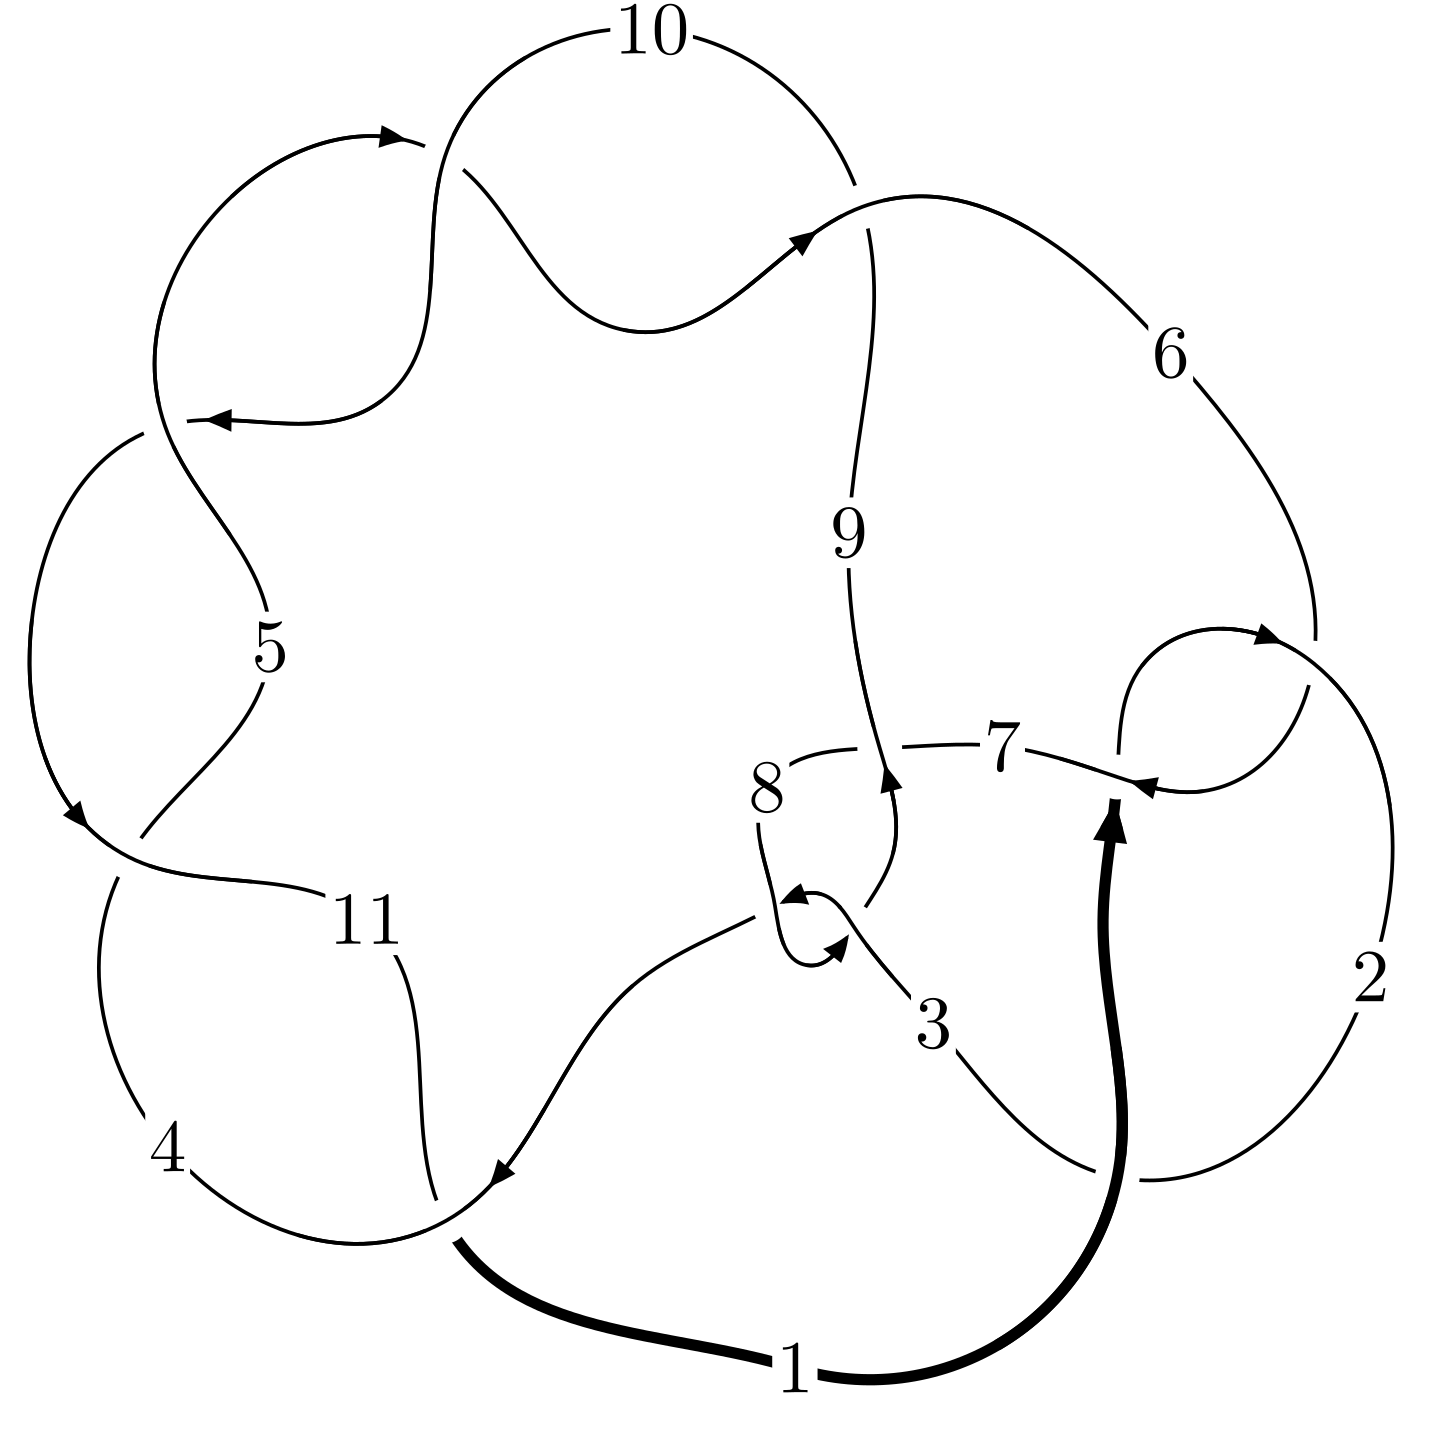
\includegraphics[width=112pt]{../../../GIT/diagram.site/Diagrams/png/463_11a_214.png}\\
\ \ \ A knot diagram\footnotemark}&
\allowdisplaybreaks
\textbf{Linearized knot diagam} \\
\cline{2-2}
 &
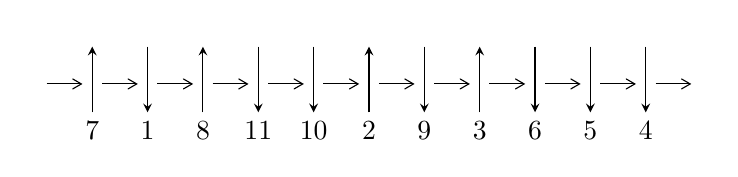
\begin{tikzpicture}[x=20pt, y=17pt]
	% nodes
	\node (C0) at (0, 0) {};
	\node (C1) at (1, 0) {};
	\node (C1U) at (1, +1) {};
	\node (C1D) at (1, -1) {7};

	\node (C2) at (2, 0) {};
	\node (C2U) at (2, +1) {};
	\node (C2D) at (2, -1) {1};

	\node (C3) at (3, 0) {};
	\node (C3U) at (3, +1) {};
	\node (C3D) at (3, -1) {8};

	\node (C4) at (4, 0) {};
	\node (C4U) at (4, +1) {};
	\node (C4D) at (4, -1) {11};

	\node (C5) at (5, 0) {};
	\node (C5U) at (5, +1) {};
	\node (C5D) at (5, -1) {10};

	\node (C6) at (6, 0) {};
	\node (C6U) at (6, +1) {};
	\node (C6D) at (6, -1) {2};

	\node (C7) at (7, 0) {};
	\node (C7U) at (7, +1) {};
	\node (C7D) at (7, -1) {9};

	\node (C8) at (8, 0) {};
	\node (C8U) at (8, +1) {};
	\node (C8D) at (8, -1) {3};

	\node (C9) at (9, 0) {};
	\node (C9U) at (9, +1) {};
	\node (C9D) at (9, -1) {6};

	\node (C10) at (10, 0) {};
	\node (C10U) at (10, +1) {};
	\node (C10D) at (10, -1) {5};

	\node (C11) at (11, 0) {};
	\node (C11U) at (11, +1) {};
	\node (C11D) at (11, -1) {4};
	\node (C12) at (12, 0) {};

	% arrows
	\draw[->,>={angle 60}]
	(C0) edge (C1) (C1) edge (C2) (C2) edge (C3) (C3) edge (C4) (C4) edge (C5) (C5) edge (C6) (C6) edge (C7) (C7) edge (C8) (C8) edge (C9) (C9) edge (C10) (C10) edge (C11) (C11) edge (C12) ;	\draw[->,>=stealth]
	(C1D) edge (C1U) (C2U) edge (C2D) (C3D) edge (C3U) (C4U) edge (C4D) (C5U) edge (C5D) (C6D) edge (C6U) (C7U) edge (C7D) (C8D) edge (C8U) (C9U) edge (C9D) (C10U) edge (C10D) (C11U) edge (C11D) ;
	\end{tikzpicture} \\
\hhline{~~} \\& 
\textbf{Solving Sequence} \\ \cline{2-2} 
 &
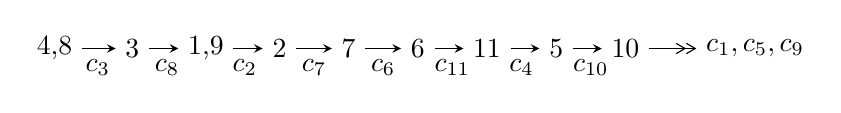
\begin{tikzpicture}[x=25pt, y=7pt]
	% node
	\node (A0) at (-1/8, 0) {4,8};
	\node (A1) at (1, 0) {3};
	\node (A2) at (33/16, 0) {1,9};
	\node (A3) at (25/8, 0) {2};
	\node (A4) at (33/8, 0) {7};
	\node (A5) at (41/8, 0) {6};
	\node (A6) at (49/8, 0) {11};
	\node (A7) at (57/8, 0) {5};
	\node (A8) at (65/8, 0) {10};
	\node (C1) at (1/2, -1) {$c_{3}$};
	\node (C2) at (3/2, -1) {$c_{8}$};
	\node (C3) at (21/8, -1) {$c_{2}$};
	\node (C4) at (29/8, -1) {$c_{7}$};
	\node (C5) at (37/8, -1) {$c_{6}$};
	\node (C6) at (45/8, -1) {$c_{11}$};
	\node (C7) at (53/8, -1) {$c_{4}$};
	\node (C8) at (61/8, -1) {$c_{10}$};
	\node (A9) at (10, 0) {$c_{1},c_{5},c_{9}$};

	% edge
	\draw[->,>=stealth]	
	(A0) edge (A1) (A1) edge (A2) (A2) edge (A3) (A3) edge (A4) (A4) edge (A5) (A5) edge (A6) (A6) edge (A7) (A7) edge (A8) ;
	\draw[->>,>={angle 60}]	
	(A8) edge (A9);
\end{tikzpicture} \\ 

\end{tabular} \\

\footnotetext{
The image of knot diagram is generated by the software ``\textbf{Draw programme}" developed by Andrew Bartholomew(\url{http://www.layer8.co.uk/maths/draw/index.htm\#Running-draw}), where we modified some parts for our purpose(\url{https://github.com/CATsTAILs/LinksPainter}).
}\phantom \\ \newline 
\centering \textbf{Ideals for irreducible components\footnotemark of $X_{\text{par}}$} 
 
\begin{align*}
I^u_{1}&=\langle 
u^{15}- u^{14}+2 u^{13}- u^{12}+5 u^{11}-5 u^{10}+4 u^9-2 u^8+7 u^7-11 u^6+4 u^5-4 u^4+5 u^3-11 u^2+4 b-1,\\
\phantom{I^u_{1}}&\phantom{= \langle  }- u^{15}+u^{14}-2 u^{13}+u^{12}-5 u^{11}+5 u^{10}-4 u^9+2 u^8-7 u^7+11 u^6-4 u^5-5 u^3+7 u^2+4 a-3,\\
\phantom{I^u_{1}}&\phantom{= \langle  }u^{16}+3 u^{14}+u^{13}+8 u^{12}+2 u^{11}+11 u^{10}+4 u^9+15 u^8+2 u^7+13 u^6+2 u^5+11 u^4+5 u^2+u+1\rangle \\
I^u_{2}&=\langle 
24532 u^{21}+99990 u^{20}+\cdots+429733 b+160508,\\
\phantom{I^u_{2}}&\phantom{= \langle  }1188174 u^{21}-128444 u^{20}+\cdots+2148665 a+5939931,\;u^{22}- u^{21}+\cdots-6 u+5\rangle \\
I^u_{3}&=\langle 
b+a+1,\;a^2- a u+2 a- u+2,\;u^2+1\rangle \\
\\
\end{align*}
\raggedright * 3 irreducible components of $\dim_{\mathbb{C}}=0$, with total 42 representations.\\
\footnotetext{All coefficients of polynomials are rational numbers. But the coefficients are sometimes approximated in decimal forms when there is not enough margin.}
\newpage
\renewcommand{\arraystretch}{1}
\centering \section*{I. $I^u_{1}= \langle u^{15}- u^{14}+\cdots+4 b-1,\;- u^{15}+u^{14}+\cdots+4 a-3,\;u^{16}+3 u^{14}+\cdots+u+1 \rangle$}
\flushleft \textbf{(i) Arc colorings}\\
\begin{tabular}{m{7pt} m{180pt} m{7pt} m{180pt} }
\flushright $a_{4}=$&$\begin{pmatrix}1\\0\end{pmatrix}$ \\
\flushright $a_{8}=$&$\begin{pmatrix}0\\u\end{pmatrix}$ \\
\flushright $a_{3}=$&$\begin{pmatrix}1\\u^2\end{pmatrix}$ \\
\flushright $a_{1}=$&$\begin{pmatrix}\frac{1}{4} u^{15}-\frac{1}{4} u^{14}+\cdots-\frac{7}{4} u^2+\frac{3}{4}\\-\frac{1}{4} u^{15}+\frac{1}{4} u^{14}+\cdots+\frac{11}{4} u^2+\frac{1}{4}\end{pmatrix}$ \\
\flushright $a_{9}=$&$\begin{pmatrix}u\\u^3+u\end{pmatrix}$ \\
\flushright $a_{2}=$&$\begin{pmatrix}\frac{1}{4} u^{15}-\frac{1}{4} u^{14}+\cdots-\frac{7}{4} u^2+\frac{3}{4}\\-\frac{1}{4} u^{15}+\frac{1}{4} u^{14}+\cdots+\frac{7}{4} u^2+\frac{1}{4}\end{pmatrix}$ \\
\flushright $a_{7}=$&$\begin{pmatrix}u^3\\u^5+u^3+u\end{pmatrix}$ \\
\flushright $a_{6}=$&$\begin{pmatrix}\frac{1}{4} u^{15}+\frac{1}{4} u^{14}+\cdots-\frac{1}{2} u+\frac{1}{4}\\-\frac{1}{4} u^{15}-\frac{1}{4} u^{14}+\cdots+\frac{1}{2} u-\frac{1}{4}\end{pmatrix}$ \\
\flushright $a_{11}=$&$\begin{pmatrix}u^4+u^2+1\\-\frac{1}{4} u^{15}+\frac{1}{4} u^{14}+\cdots+\frac{11}{4} u^2+\frac{1}{4}\end{pmatrix}$ \\
\flushright $a_{5}=$&$\begin{pmatrix}-\frac{1}{4} u^{15}+\frac{1}{4} u^{14}+\cdots+\frac{11}{4} u^2+\frac{5}{4}\\u^{15}+\frac{5}{2} u^{13}+\cdots+u-\frac{1}{2}\end{pmatrix}$ \\
\flushright $a_{10}=$&$\begin{pmatrix}\frac{1}{4} u^{15}+\frac{3}{4} u^{14}+\cdots+u+\frac{5}{4}\\-\frac{1}{2} u^{14}-\frac{1}{2} u^{13}+\cdots-\frac{5}{2} u-1\end{pmatrix}$\\ \flushright $a_{10}=$&$\begin{pmatrix}\frac{1}{4} u^{15}+\frac{3}{4} u^{14}+\cdots+u+\frac{5}{4}\\-\frac{1}{2} u^{14}-\frac{1}{2} u^{13}+\cdots-\frac{5}{2} u-1\end{pmatrix}$\\&\end{tabular}
\flushleft \textbf{(ii) Obstruction class $= -1$}\\~\\
\flushleft \textbf{(iii) Cusp Shapes $= 3 u^{15}-2 u^{14}+9 u^{13}-2 u^{12}+21 u^{11}-9 u^{10}+27 u^9-8 u^8+32 u^7-26 u^6+30 u^5-17 u^4+23 u^3-23 u^2+11 u-3$}\\~\\
\newpage\renewcommand{\arraystretch}{1}
\flushleft \textbf{(iv) u-Polynomials at the component}\newline \\
\begin{tabular}{m{50pt}|m{274pt}}
Crossings & \hspace{64pt}u-Polynomials at each crossing \\
\hline $$\begin{aligned}c_{1},c_{3},c_{6}\\c_{8}\end{aligned}$$&$\begin{aligned}
&u^{16}+3 u^{14}+\cdots- u+1
\end{aligned}$\\
\hline $$\begin{aligned}c_{2},c_{7}\end{aligned}$$&$\begin{aligned}
&u^{16}+6 u^{15}+\cdots+9 u+1
\end{aligned}$\\
\hline $$\begin{aligned}c_{4},c_{5},c_{9}\\c_{10},c_{11}\end{aligned}$$&$\begin{aligned}
&u^{16}-3 u^{15}+\cdots-7 u+2
\end{aligned}$\\
\hline
\end{tabular}\\~\\
\newpage\renewcommand{\arraystretch}{1}
\flushleft \textbf{(v) Riley Polynomials at the component}\newline \\
\begin{tabular}{m{50pt}|m{274pt}}
Crossings & \hspace{64pt}Riley Polynomials at each crossing \\
\hline $$\begin{aligned}c_{1},c_{3},c_{6}\\c_{8}\end{aligned}$$&$\begin{aligned}
&y^{16}+6 y^{15}+\cdots+9 y+1
\end{aligned}$\\
\hline $$\begin{aligned}c_{2},c_{7}\end{aligned}$$&$\begin{aligned}
&y^{16}+14 y^{15}+\cdots+13 y+1
\end{aligned}$\\
\hline $$\begin{aligned}c_{4},c_{5},c_{9}\\c_{10},c_{11}\end{aligned}$$&$\begin{aligned}
&y^{16}+21 y^{15}+\cdots+23 y+4
\end{aligned}$\\
\hline
\end{tabular}\\~\\
\newpage\flushleft \textbf{(vi) Complex Volumes and Cusp Shapes}
$$\begin{array}{c|c|c}  
\text{Solutions to }I^u_{1}& \I (\text{vol} + \sqrt{-1}CS) & \text{Cusp shape}\\
 \hline 
\begin{aligned}
u &= \phantom{-}0.739034 + 0.627334 I \\
a &= \phantom{-}0.206056 + 0.079796 I \\
b &= \phantom{-}0.110083 + 1.130490 I\end{aligned}
 & \phantom{-}5.48130 + 1.05317 I & \phantom{-}4.45688 - 2.38990 I \\ \hline\begin{aligned}
u &= \phantom{-}0.739034 - 0.627334 I \\
a &= \phantom{-}0.206056 - 0.079796 I \\
b &= \phantom{-}0.110083 - 1.130490 I\end{aligned}
 & \phantom{-}5.48130 - 1.05317 I & \phantom{-}4.45688 + 2.38990 I \\ \hline\begin{aligned}
u &= -0.555046 + 0.909908 I \\
a &= -0.752118 + 0.605011 I \\
b &= \phantom{-}0.482247 - 0.564899 I\end{aligned}
 & -0.19881 - 2.75301 I & -1.57245 + 2.26508 I \\ \hline\begin{aligned}
u &= -0.555046 - 0.909908 I \\
a &= -0.752118 - 0.605011 I \\
b &= \phantom{-}0.482247 + 0.564899 I\end{aligned}
 & -0.19881 + 2.75301 I & -1.57245 - 2.26508 I \\ \hline\begin{aligned}
u &= -0.926846 + 0.626361 I \\
a &= \phantom{-}0.304991 - 0.497485 I \\
b &= \phantom{-}0.03144 - 1.74738 I\end{aligned}
 & \phantom{-}15.8152 - 0.4292 I & \phantom{-}4.82755 + 2.00465 I \\ \hline\begin{aligned}
u &= -0.926846 - 0.626361 I \\
a &= \phantom{-}0.304991 + 0.497485 I \\
b &= \phantom{-}0.03144 + 1.74738 I\end{aligned}
 & \phantom{-}15.8152 + 0.4292 I & \phantom{-}4.82755 - 2.00465 I \\ \hline\begin{aligned}
u &= \phantom{-}0.317155 + 0.789225 I \\
a &= \phantom{-}0.47307 - 1.59041 I \\
b &= \phantom{-}0.02681 + 1.56809 I\end{aligned}
 & \phantom{-}6.59915 + 1.30998 I & \phantom{-}1.95561 - 5.45778 I \\ \hline\begin{aligned}
u &= \phantom{-}0.317155 - 0.789225 I \\
a &= \phantom{-}0.47307 + 1.59041 I \\
b &= \phantom{-}0.02681 - 1.56809 I\end{aligned}
 & \phantom{-}6.59915 - 1.30998 I & \phantom{-}1.95561 + 5.45778 I \\ \hline\begin{aligned}
u &= \phantom{-}0.596655 + 1.032140 I \\
a &= -1.346280 - 0.306488 I \\
b &= \phantom{-}0.623112 - 0.209109 I\end{aligned}
 & -1.29053 + 6.45307 I & -4.44807 - 7.45131 I \\ \hline\begin{aligned}
u &= \phantom{-}0.596655 - 1.032140 I \\
a &= -1.346280 + 0.306488 I \\
b &= \phantom{-}0.623112 + 0.209109 I\end{aligned}
 & -1.29053 - 6.45307 I & -4.44807 + 7.45131 I\\
 \hline 
 \end{array}$$\newpage$$\begin{array}{c|c|c}  
\text{Solutions to }I^u_{1}& \I (\text{vol} + \sqrt{-1}CS) & \text{Cusp shape}\\
 \hline 
\begin{aligned}
u &= -0.652805 + 1.114230 I \\
a &= -1.64360 - 0.10173 I \\
b &= \phantom{-}0.376764 + 1.019230 I\end{aligned}
 & \phantom{-}2.50481 - 9.84228 I & -0.10556 + 8.25112 I \\ \hline\begin{aligned}
u &= -0.652805 - 1.114230 I \\
a &= -1.64360 + 0.10173 I \\
b &= \phantom{-}0.376764 - 1.019230 I\end{aligned}
 & \phantom{-}2.50481 + 9.84228 I & -0.10556 - 8.25112 I \\ \hline\begin{aligned}
u &= \phantom{-}0.691623 + 1.176670 I \\
a &= -1.83564 + 0.40291 I \\
b &= \phantom{-}0.10149 - 1.72523 I\end{aligned}
 & \phantom{-}12.2077 + 11.7947 I & \phantom{-}0.96071 - 6.63599 I \\ \hline\begin{aligned}
u &= \phantom{-}0.691623 - 1.176670 I \\
a &= -1.83564 - 0.40291 I \\
b &= \phantom{-}0.10149 + 1.72523 I\end{aligned}
 & \phantom{-}12.2077 - 11.7947 I & \phantom{-}0.96071 + 6.63599 I \\ \hline\begin{aligned}
u &= -0.209770 + 0.436269 I \\
a &= \phantom{-}1.093530 + 0.297205 I \\
b &= -0.251943 - 0.426672 I\end{aligned}
 & \phantom{-}0.004513 - 0.990902 I & -0.07468 + 7.34190 I \\ \hline\begin{aligned}
u &= -0.209770 - 0.436269 I \\
a &= \phantom{-}1.093530 - 0.297205 I \\
b &= -0.251943 + 0.426672 I\end{aligned}
 & \phantom{-}0.004513 + 0.990902 I & -0.07468 - 7.34190 I\\
 \hline 
 \end{array}$$\newpage\newpage\renewcommand{\arraystretch}{1}
\centering \section*{II. $I^u_{2}= \langle 24532 u^{21}+99990 u^{20}+\cdots+429733 b+160508,\;1.19\times10^{6} u^{21}-1.28\times10^{5} u^{20}+\cdots+2.15\times10^{6} a+5.94\times10^{6},\;u^{22}- u^{21}+\cdots-6 u+5 \rangle$}
\flushleft \textbf{(i) Arc colorings}\\
\begin{tabular}{m{7pt} m{180pt} m{7pt} m{180pt} }
\flushright $a_{4}=$&$\begin{pmatrix}1\\0\end{pmatrix}$ \\
\flushright $a_{8}=$&$\begin{pmatrix}0\\u\end{pmatrix}$ \\
\flushright $a_{3}=$&$\begin{pmatrix}1\\u^2\end{pmatrix}$ \\
\flushright $a_{1}=$&$\begin{pmatrix}-0.552982 u^{21}+0.0597785 u^{20}+\cdots+1.60210 u-2.76448\\-0.0570866 u^{21}-0.232679 u^{20}+\cdots+0.277416 u-0.373506\end{pmatrix}$ \\
\flushright $a_{9}=$&$\begin{pmatrix}u\\u^3+u\end{pmatrix}$ \\
\flushright $a_{2}=$&$\begin{pmatrix}-0.610069 u^{21}-0.172901 u^{20}+\cdots+1.87951 u-2.13798\\-0.295974 u^{21}-0.109836 u^{20}+\cdots-0.426602 u-0.137709\end{pmatrix}$ \\
\flushright $a_{7}=$&$\begin{pmatrix}u^3\\u^5+u^3+u\end{pmatrix}$ \\
\flushright $a_{6}=$&$\begin{pmatrix}-0.857671 u^{21}+1.08755 u^{20}+\cdots-5.92382 u+3.22114\\-0.358651 u^{21}+0.737100 u^{20}+\cdots-1.13075 u+1.90093\end{pmatrix}$ \\
\flushright $a_{11}=$&$\begin{pmatrix}-0.610069 u^{21}-0.172901 u^{20}+\cdots+1.87951 u-3.13798\\-0.0570866 u^{21}-0.232679 u^{20}+\cdots+0.277416 u-0.373506\end{pmatrix}$ \\
\flushright $a_{5}=$&$\begin{pmatrix}0.297712 u^{21}-0.0832768 u^{20}+\cdots+0.722951 u-1.80592\\-0.0824745 u^{21}-0.0617407 u^{20}+\cdots+0.677572 u-1.65554\end{pmatrix}$ \\
\flushright $a_{10}=$&$\begin{pmatrix}0.116673 u^{21}+0.386783 u^{20}+\cdots+2.80778 u+0.179480\\0.531833 u^{21}-0.160528 u^{20}+\cdots+2.45702 u-1.02872\end{pmatrix}$\\ \flushright $a_{10}=$&$\begin{pmatrix}0.116673 u^{21}+0.386783 u^{20}+\cdots+2.80778 u+0.179480\\0.531833 u^{21}-0.160528 u^{20}+\cdots+2.45702 u-1.02872\end{pmatrix}$\\&\end{tabular}
\flushleft \textbf{(ii) Obstruction class $= -1$}\\~\\
\flushleft \textbf{(iii) Cusp Shapes $= -\frac{412776}{429733} u^{21}-\frac{136152}{429733} u^{20}+\cdots+\frac{1938508}{429733} u-\frac{1667194}{429733}$}\\~\\
\newpage\renewcommand{\arraystretch}{1}
\flushleft \textbf{(iv) u-Polynomials at the component}\newline \\
\begin{tabular}{m{50pt}|m{274pt}}
Crossings & \hspace{64pt}u-Polynomials at each crossing \\
\hline $$\begin{aligned}c_{1},c_{3},c_{6}\\c_{8}\end{aligned}$$&$\begin{aligned}
&u^{22}+u^{21}+\cdots+6 u+5
\end{aligned}$\\
\hline $$\begin{aligned}c_{2},c_{7}\end{aligned}$$&$\begin{aligned}
&u^{22}+11 u^{21}+\cdots+124 u+25
\end{aligned}$\\
\hline $$\begin{aligned}c_{4},c_{5},c_{9}\\c_{10},c_{11}\end{aligned}$$&$\begin{aligned}
&(u^{11}+u^{10}+8 u^9+7 u^8+22 u^7+16 u^6+24 u^5+13 u^4+9 u^3+3 u^2-1)^2
\end{aligned}$\\
\hline
\end{tabular}\\~\\
\newpage\renewcommand{\arraystretch}{1}
\flushleft \textbf{(v) Riley Polynomials at the component}\newline \\
\begin{tabular}{m{50pt}|m{274pt}}
Crossings & \hspace{64pt}Riley Polynomials at each crossing \\
\hline $$\begin{aligned}c_{1},c_{3},c_{6}\\c_{8}\end{aligned}$$&$\begin{aligned}
&y^{22}+11 y^{21}+\cdots+124 y+25
\end{aligned}$\\
\hline $$\begin{aligned}c_{2},c_{7}\end{aligned}$$&$\begin{aligned}
&y^{22}- y^{21}+\cdots+4824 y+625
\end{aligned}$\\
\hline $$\begin{aligned}c_{4},c_{5},c_{9}\\c_{10},c_{11}\end{aligned}$$&$\begin{aligned}
&(y^{11}+15 y^{10}+\cdots+6 y-1)^{2}
\end{aligned}$\\
\hline
\end{tabular}\\~\\
\newpage\flushleft \textbf{(vi) Complex Volumes and Cusp Shapes}
$$\begin{array}{c|c|c}  
\text{Solutions to }I^u_{2}& \I (\text{vol} + \sqrt{-1}CS) & \text{Cusp shape}\\
 \hline 
\begin{aligned}
u &= \phantom{-}0.579803 + 0.857238 I \\
a &= -1.85524 - 1.12681 I \\
b &= \phantom{-}0.03037 - 1.69780 I\end{aligned}
 & \phantom{-}7.95553 + 2.30219 I & \phantom{-}0.32022 - 2.86330 I \\ \hline\begin{aligned}
u &= \phantom{-}0.579803 - 0.857238 I \\
a &= -1.85524 + 1.12681 I \\
b &= \phantom{-}0.03037 + 1.69780 I\end{aligned}
 & \phantom{-}7.95553 - 2.30219 I & \phantom{-}0.32022 + 2.86330 I \\ \hline\begin{aligned}
u &= -0.399913 + 0.875160 I \\
a &= -1.65574 + 0.96794 I \\
b &= \phantom{-}0.147502 + 0.884325 I\end{aligned}
 & -1.26759 - 1.65848 I & -0.54419 + 4.72916 I \\ \hline\begin{aligned}
u &= -0.399913 - 0.875160 I \\
a &= -1.65574 - 0.96794 I \\
b &= \phantom{-}0.147502 - 0.884325 I\end{aligned}
 & -1.26759 + 1.65848 I & -0.54419 - 4.72916 I \\ \hline\begin{aligned}
u &= -0.529162 + 0.802687 I \\
a &= \phantom{-}1.204780 - 0.193673 I \\
b &= -0.499488 - 0.319159 I\end{aligned}
 & \phantom{-}0.18031 - 1.62554 I & -1.42199 + 3.91435 I \\ \hline\begin{aligned}
u &= -0.529162 - 0.802687 I \\
a &= \phantom{-}1.204780 + 0.193673 I \\
b &= -0.499488 + 0.319159 I\end{aligned}
 & \phantom{-}0.18031 + 1.62554 I & -1.42199 - 3.91435 I \\ \hline\begin{aligned}
u &= -0.848321 + 0.450725 I \\
a &= \phantom{-}0.353490 + 0.072972 I \\
b &= -0.275765 + 1.061690 I\end{aligned}
 & \phantom{-}4.47712 + 4.26374 I & \phantom{-}2.95029 - 4.02329 I \\ \hline\begin{aligned}
u &= -0.848321 - 0.450725 I \\
a &= \phantom{-}0.353490 - 0.072972 I \\
b &= -0.275765 - 1.061690 I\end{aligned}
 & \phantom{-}4.47712 - 4.26374 I & \phantom{-}2.95029 + 4.02329 I \\ \hline\begin{aligned}
u &= \phantom{-}0.197868 + 1.057100 I \\
a &= -1.010600 - 0.780021 I \\
b &= \phantom{-}0.337740\phantom{ +0.000000I}\end{aligned}
 & -3.92670\phantom{ +0.000000I} & -11.69818 + 0. I\phantom{ +0.000000I} \\ \hline\begin{aligned}
u &= \phantom{-}0.197868 - 1.057100 I \\
a &= -1.010600 + 0.780021 I \\
b &= \phantom{-}0.337740\phantom{ +0.000000I}\end{aligned}
 & -3.92670\phantom{ +0.000000I} & -11.69818 + 0. I\phantom{ +0.000000I}\\
 \hline 
 \end{array}$$\newpage$$\begin{array}{c|c|c}  
\text{Solutions to }I^u_{2}& \I (\text{vol} + \sqrt{-1}CS) & \text{Cusp shape}\\
 \hline 
\begin{aligned}
u &= \phantom{-}0.986171 + 0.439556 I \\
a &= \phantom{-}0.194359 - 0.406737 I \\
b &= -0.07149 - 1.73688 I\end{aligned}
 & \phantom{-}14.4695 - 5.6984 I & \phantom{-}3.54476 + 2.83577 I \\ \hline\begin{aligned}
u &= \phantom{-}0.986171 - 0.439556 I \\
a &= \phantom{-}0.194359 + 0.406737 I \\
b &= -0.07149 + 1.73688 I\end{aligned}
 & \phantom{-}14.4695 + 5.6984 I & \phantom{-}3.54476 - 2.83577 I \\ \hline\begin{aligned}
u &= \phantom{-}0.662778 + 0.976432 I \\
a &= \phantom{-}1.42879 + 0.04455 I \\
b &= -0.275765 + 1.061690 I\end{aligned}
 & \phantom{-}4.47712 + 4.26374 I & \phantom{-}2.95029 - 4.02329 I \\ \hline\begin{aligned}
u &= \phantom{-}0.662778 - 0.976432 I \\
a &= \phantom{-}1.42879 - 0.04455 I \\
b &= -0.275765 - 1.061690 I\end{aligned}
 & \phantom{-}4.47712 - 4.26374 I & \phantom{-}2.95029 + 4.02329 I \\ \hline\begin{aligned}
u &= \phantom{-}0.610796 + 0.518790 I \\
a &= \phantom{-}0.780853 + 0.341379 I \\
b &= -0.499488 - 0.319159 I\end{aligned}
 & \phantom{-}0.18031 - 1.62554 I & -1.42199 + 3.91435 I \\ \hline\begin{aligned}
u &= \phantom{-}0.610796 - 0.518790 I \\
a &= \phantom{-}0.780853 - 0.341379 I \\
b &= -0.499488 + 0.319159 I\end{aligned}
 & \phantom{-}0.18031 + 1.62554 I & -1.42199 - 3.91435 I \\ \hline\begin{aligned}
u &= -0.125296 + 1.244620 I \\
a &= -0.270054 + 1.088140 I \\
b &= \phantom{-}0.147502 - 0.884325 I\end{aligned}
 & -1.26759 + 1.65848 I & -0.54419 - 4.72916 I \\ \hline\begin{aligned}
u &= -0.125296 - 1.244620 I \\
a &= -0.270054 - 1.088140 I \\
b &= \phantom{-}0.147502 + 0.884325 I\end{aligned}
 & -1.26759 - 1.65848 I & -0.54419 + 4.72916 I \\ \hline\begin{aligned}
u &= -0.746289 + 1.064200 I \\
a &= \phantom{-}1.62058 + 0.05160 I \\
b &= -0.07149 - 1.73688 I\end{aligned}
 & \phantom{-}14.4695 - 5.6984 I & \phantom{-}3.54476 + 2.83577 I \\ \hline\begin{aligned}
u &= -0.746289 - 1.064200 I \\
a &= \phantom{-}1.62058 - 0.05160 I \\
b &= -0.07149 + 1.73688 I\end{aligned}
 & \phantom{-}14.4695 + 5.6984 I & \phantom{-}3.54476 - 2.83577 I\\
 \hline 
 \end{array}$$\newpage$$\begin{array}{c|c|c}  
\text{Solutions to }I^u_{2}& \I (\text{vol} + \sqrt{-1}CS) & \text{Cusp shape}\\
 \hline 
\begin{aligned}
u &= \phantom{-}0.111564 + 1.357150 I \\
a &= \phantom{-}0.00879 - 1.46999 I \\
b &= \phantom{-}0.03037 + 1.69780 I\end{aligned}
 & \phantom{-}7.95553 - 2.30219 I & \phantom{-}0.32022 + 2.86330 I \\ \hline\begin{aligned}
u &= \phantom{-}0.111564 - 1.357150 I \\
a &= \phantom{-}0.00879 + 1.46999 I \\
b &= \phantom{-}0.03037 - 1.69780 I\end{aligned}
 & \phantom{-}7.95553 + 2.30219 I & \phantom{-}0.32022 - 2.86330 I\\
 \hline 
 \end{array}$$\newpage\newpage\renewcommand{\arraystretch}{1}
\centering \section*{III. $I^u_{3}= \langle b+a+1,\;a^2- a u+2 a- u+2,\;u^2+1 \rangle$}
\flushleft \textbf{(i) Arc colorings}\\
\begin{tabular}{m{7pt} m{180pt} m{7pt} m{180pt} }
\flushright $a_{4}=$&$\begin{pmatrix}1\\0\end{pmatrix}$ \\
\flushright $a_{8}=$&$\begin{pmatrix}0\\u\end{pmatrix}$ \\
\flushright $a_{3}=$&$\begin{pmatrix}1\\-1\end{pmatrix}$ \\
\flushright $a_{1}=$&$\begin{pmatrix}a\\- a-1\end{pmatrix}$ \\
\flushright $a_{9}=$&$\begin{pmatrix}u\\0\end{pmatrix}$ \\
\flushright $a_{2}=$&$\begin{pmatrix}a+1\\- a-2\end{pmatrix}$ \\
\flushright $a_{7}=$&$\begin{pmatrix}- u\\u\end{pmatrix}$ \\
\flushright $a_{6}=$&$\begin{pmatrix}a u\\- a u- u\end{pmatrix}$ \\
\flushright $a_{11}=$&$\begin{pmatrix}-1\\- a-1\end{pmatrix}$ \\
\flushright $a_{5}=$&$\begin{pmatrix}a+2\\a u+u-1\end{pmatrix}$ \\
\flushright $a_{10}=$&$\begin{pmatrix}- a u- a- u-1\\a+u+1\end{pmatrix}$\\ \flushright $a_{10}=$&$\begin{pmatrix}- a u- a- u-1\\a+u+1\end{pmatrix}$\\&\end{tabular}
\flushleft \textbf{(ii) Obstruction class $= 1$}\\~\\
\flushleft \textbf{(iii) Cusp Shapes $= -4$}\\~\\
\newpage\renewcommand{\arraystretch}{1}
\flushleft \textbf{(iv) u-Polynomials at the component}\newline \\
\begin{tabular}{m{50pt}|m{274pt}}
Crossings & \hspace{64pt}u-Polynomials at each crossing \\
\hline $$\begin{aligned}c_{1},c_{3},c_{6}\\c_{8}\end{aligned}$$&$\begin{aligned}
&(u^2+1)^2
\end{aligned}$\\
\hline $$\begin{aligned}c_{2}\end{aligned}$$&$\begin{aligned}
&(u+1)^4
\end{aligned}$\\
\hline $$\begin{aligned}c_{4},c_{5},c_{9}\\c_{10},c_{11}\end{aligned}$$&$\begin{aligned}
&u^4+3 u^2+1
\end{aligned}$\\
\hline $$\begin{aligned}c_{7}\end{aligned}$$&$\begin{aligned}
&(u-1)^4
\end{aligned}$\\
\hline
\end{tabular}\\~\\
\newpage\renewcommand{\arraystretch}{1}
\flushleft \textbf{(v) Riley Polynomials at the component}\newline \\
\begin{tabular}{m{50pt}|m{274pt}}
Crossings & \hspace{64pt}Riley Polynomials at each crossing \\
\hline $$\begin{aligned}c_{1},c_{3},c_{6}\\c_{8}\end{aligned}$$&$\begin{aligned}
&(y+1)^4
\end{aligned}$\\
\hline $$\begin{aligned}c_{2},c_{7}\end{aligned}$$&$\begin{aligned}
&(y-1)^4
\end{aligned}$\\
\hline $$\begin{aligned}c_{4},c_{5},c_{9}\\c_{10},c_{11}\end{aligned}$$&$\begin{aligned}
&(y^2+3 y+1)^2
\end{aligned}$\\
\hline
\end{tabular}\\~\\
\newpage\flushleft \textbf{(vi) Complex Volumes and Cusp Shapes}
$$\begin{array}{c|c|c}  
\text{Solutions to }I^u_{3}& \I (\text{vol} + \sqrt{-1}CS) & \text{Cusp shape}\\
 \hline 
\begin{aligned}
u &= \phantom{-0.000000 -}1.000000 I \\
a &= -1.000000 - 0.618034 I \\
b &= \phantom{-0.000000 -}0.618034 I\end{aligned}
 & -2.30291\phantom{ +0.000000I} & -4.00000\phantom{ +0.000000I} \\ \hline\begin{aligned}
u &= \phantom{-0.000000 -}1.000000 I \\
a &= -1.00000 + 1.61803 I \\
b &= \phantom{-0.000000 } -1.61803 I\end{aligned}
 & \phantom{-}5.59278\phantom{ +0.000000I} & -4.00000\phantom{ +0.000000I} \\ \hline\begin{aligned}
u &= \phantom{-0.000000 } -1.000000 I \\
a &= -1.000000 + 0.618034 I \\
b &= \phantom{-0.000000 } -0.618034 I\end{aligned}
 & -2.30291\phantom{ +0.000000I} & -4.00000\phantom{ +0.000000I} \\ \hline\begin{aligned}
u &= \phantom{-0.000000 } -1.000000 I \\
a &= -1.00000 - 1.61803 I \\
b &= \phantom{-0.000000 -}1.61803 I\end{aligned}
 & \phantom{-}5.59278\phantom{ +0.000000I} & -4.00000\phantom{ +0.000000I}\\
 \hline 
 \end{array}$$\newpage
\newpage\renewcommand{\arraystretch}{1}
\centering \section*{ IV. u-Polynomials}
\begin{tabular}{m{50pt}|m{274pt}}
Crossings & \hspace{64pt}u-Polynomials at each crossing \\
\hline $$\begin{aligned}c_{1},c_{3},c_{6}\\c_{8}\end{aligned}$$&$\begin{aligned}
&((u^2+1)^2)(u^{16}+3 u^{14}+\cdots- u+1)(u^{22}+u^{21}+\cdots+6 u+5)
\end{aligned}$\\
\hline $$\begin{aligned}c_{2}\end{aligned}$$&$\begin{aligned}
&((u+1)^4)(u^{16}+6 u^{15}+\cdots+9 u+1)(u^{22}+11 u^{21}+\cdots+124 u+25)
\end{aligned}$\\
\hline $$\begin{aligned}c_{4},c_{5},c_{9}\\c_{10},c_{11}\end{aligned}$$&$\begin{aligned}
&(u^4+3 u^2+1)\\
&\cdot(u^{11}+u^{10}+8 u^9+7 u^8+22 u^7+16 u^6+24 u^5+13 u^4+9 u^3+3 u^2-1)^2\\
&\cdot(u^{16}-3 u^{15}+\cdots-7 u+2)
\end{aligned}$\\
\hline $$\begin{aligned}c_{7}\end{aligned}$$&$\begin{aligned}
&((u-1)^4)(u^{16}+6 u^{15}+\cdots+9 u+1)(u^{22}+11 u^{21}+\cdots+124 u+25)
\end{aligned}$\\
\hline
\end{tabular}\newpage\renewcommand{\arraystretch}{1}
\centering \section*{ V. Riley Polynomials}
\begin{tabular}{m{50pt}|m{274pt}}
Crossings & \hspace{64pt}Riley Polynomials at each crossing \\
\hline $$\begin{aligned}c_{1},c_{3},c_{6}\\c_{8}\end{aligned}$$&$\begin{aligned}
&((y+1)^4)(y^{16}+6 y^{15}+\cdots+9 y+1)(y^{22}+11 y^{21}+\cdots+124 y+25)
\end{aligned}$\\
\hline $$\begin{aligned}c_{2},c_{7}\end{aligned}$$&$\begin{aligned}
&((y-1)^4)(y^{16}+14 y^{15}+\cdots+13 y+1)(y^{22}-y^{21}+\cdots+4824 y+625)
\end{aligned}$\\
\hline $$\begin{aligned}c_{4},c_{5},c_{9}\\c_{10},c_{11}\end{aligned}$$&$\begin{aligned}
&((y^2+3 y+1)^2)(y^{11}+15 y^{10}+\cdots+6 y-1)^{2}\\
&\cdot(y^{16}+21 y^{15}+\cdots+23 y+4)
\end{aligned}$\\
\hline
\end{tabular}
\vskip 2pc
\end{document}